\documentclass{article}
\usepackage[left=2cm,right=2cm,top=2cm,bottom=2cm]{geometry}
\usepackage[utf8]{inputenc}
\usepackage[german]{babel}
\usepackage{amsmath}
\usepackage{dsfont}
\usepackage[export]{adjustbox}
\usepackage{amsthm}
\usepackage{color}
\usepackage{amsfonts}
\usepackage{amssymb}
\usepackage{wasysym}
\usepackage{makeidx}
\usepackage{graphicx}
\usepackage[colorlinks=true,urlcolor=blue,linkcolor=blue]{hyperref}
\usepackage{ziffer}
\usepackage{minted}
\usepackage{xcolor}
\usepackage{framed}
\usepackage{mdframed}
\usepackage{subfiles}
\usemintedstyle{emacs}

\definecolor{purp}{HTML}{9A72AC}
\definecolor{re}{HTML}{FC6255}
\definecolor{gre}{HTML}{83C167}
\definecolor{blu}{HTML}{58C4DD}
\definecolor{shadecolor}{rgb}{0.85,0.85,0.85}
\definecolor{bg}{rgb}{0.95,0.95,0.95}
\setlength{\parindent}{0em} 

\BeforeBeginEnvironment{minted}{\begin{mdframed}[linewidth =2 ,backgroundcolor=bg , linecolor=black, linewidth=0.5]}
\AfterEndEnvironment{minted}{\end{mdframed}}

\newtheorem{defi}{Definition}
\BeforeBeginEnvironment{defi}{\begin{mdframed}[linewidth =2 ,backgroundcolor=bg , linecolor=black, linewidth=0.5]}
\AfterEndEnvironment{defi}{\end{mdframed}}

\newcommand{\bsp}{\textbf{Beispiel}:}
%\newcommand{\task}{\textbf{Aufgabe}:}

\newcommand{\bol}[1]{\textbf{#1}}
\newcommand{\q}[1]{\glqq #1\grqq}
\newcommand{\DODO}[1]{\textbf{\textcolor{red}{DODO:}} #1 \\ \begin{center}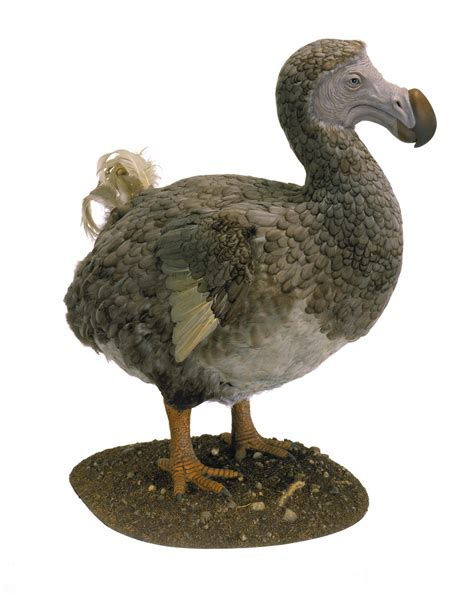
\includegraphics[scale=0.2]{../../media/dodo.jpg} \end{center}}

\newenvironment{task}[1]{
    \begin{shaded*}
    \textbf{Aufgabe #1}:
}{
    \end{shaded*}
}

\begin{document}
\subsection{Grundlagen der Softwaretechnik}
In diesem Kapitel soll es nicht mehr um Projekte gehen, die jeder Einzelne alleine angehen kann, sondern um das \q{Programmieren im Großen} - sei es in einer (internationalen) Firma oder \q{privat} in einem Verbund mit anderen Programmierys. \\
Gerade in großen Projekten ist eine qualitativ hochwertig Zusammenarbeit unerlässlich. Leider gibt es hier immer wieder große Reibungsverluste, neben den fachlichen Inhalten ist die Fähigkeit des \q{Teamwork} - gerade heutzutage - ein immens wichtiger \q{soft skill}. \\
In der Informatik gibt es verschiedene Modelle, die die Projektorganisation strukturieren und z.T. veranschaulichen sollen (dazu gibt es ganze eigene Vorlesungen im Bereich der \textbf{Softwaretechnik}!). \\
Im Allgemeinen geht man grob von den folgenden Phasen im Leben eines Softwareprojekts aus:
\begin{enumerate}
    \item Anforderungen und Spezifikationen
    \item Planung
    \item Entwurf und Design
    \item Implementierung und Integration
    \item Betrieb und Wartung
    \item Stilllegung
\end{enumerate}
Zur Beschreibung dieser Phasen, deren Interaktion und zeitlicher Abfolge gibt es verschiedenste Vorgehensodelle, von denen in folgenden Kapiteln einige vorgestellt werden sollen. \\
Zunächst aber noch Details zu den einzelnen Phasen \\
\subsection{Der Lebenszyklus von Software}
\textbf{Anforderungen und Spezifikationen} \\
Grundlegende Fragen, die eine Anforderungsanalyse zu Beginn eines Projektes beantworten sollte, sind z.B.:
\begin{itemize}
    \item welches Problem soll konkret gelöst werden?
    \item welche Leistung soll das geplante Projekt erbringen?
    \item welche Personen müssen mit einbezogen werden?
    \item gibt es sich widersprechende Anforderungen verschiedener Personen/Gruppen?
\end{itemize}
Insbesondere die letzten beiden Punkte sollen verdeutlichen, dass gerade aus Kundensicht nicht immer Einigkeit über den Funktionsumfang oder die genauen Spezifikationen eines Programs herrscht. Eine genaue Spezifikation der zu erbringenden Leistung ist deshalb wichtig, um Unzufriedenheit diesbezüglich vorzubeugen. \\
Die Anforderungsanalyse beschränkt sich aber nicht nur auf konkrete Funktionalität, sondern bildet ein ganzes Spektrum an Faktoren ab:
\begin{itemize}
    \item \textbf{Funktionale Anforderungen}: das was man zunächst erwarten würde - welche Funktion soll das System haben, wie soll es sich verhalten, etc. 
    \item \textbf{Nichtfunktionale Anforderungen}: hier geht es eher um den eigentlichen Betrieb der Software, wie leistungsfähig soll Sie sein - d.h. wie groß sind die Anforderungen an Speicher/Prozessor im laufenden Betrieb, ist die Software skalierbar, etc. 
    \item \textbf{Designbedingungen}: gibt es bereits weitere technische Bedingungen, das könnte z.B. bereits existierende Software sein, zu der Schnittstellen vorhanden bzw. eine Kompatibilität hergestellt werden muss. 
    \item \textbf{Prozessbedingungen}: dies sind eher interne Anforderungen der Entwickler - wie viele Personen sind notwendig, wie soll die Vorgehensweise bei der Entwicklung sein (zwar intern zu sehen, aber insbesondere auch der Kontakt mit dem Kunden - Ablieferung eines \q{fertigen} Produkts oder Zwischenstände z.B.). 
\end{itemize}
Übliche Verfahren, die zur Ermittlung der Anforderungen verwendet werden sind z.B. Fragebögen, Interviews, Simulationsmodelle, Workshops, etc.  \\
Die Ergebnisse müssen natürlich verschriftlicht werden, der Auftraggeber fasst alles im sogenannten \textbf{Lastenheft} zusammen, das möglichst konkret die Gesamtheit aller Anforderungen beschreibt - kurz gesagt: \textbf{Was soll erstellt werden?}. \\
Das \textbf{Pflichtenheft} dagegen beschreibt - ebenfalls möglichst konkret - wie der Auftragnehmer die Anforderungen des Auftraggebers lösen möchte, kurz: \textbf{Wie und womit wird umgesetzt}. Erst nach Akzeptanz des Pflichtenhefts beginnt die eigentliche Umsetzung. \\
\textit{Hinweis:} Diese Beschreibung entspricht in der Realität natürlich nicht immer den Gegebenheiten, sondern eher eine etwas akademische Sicht auf die Dinge. Gerade Software-Entwicklung ist ein sehr dynamischer Prozess und lässt sich selten gut in statische Kategorien verpacken. Die Schule kann hier kein sicheres aktuelles Bild vermitteln, da Regeln und Abläufe ggf. in den Betrieben bereits überholt sind $\Rightarrow$ Praktika deutlich nützlicher, um zu lernen \q{wie der Hase läuft}. \vspace{3mm} \\
\end{document}